\chapter{Extraction de caractéristiques}
\section{Courbure}

Dans ce premier exercice, nous devons implémenter la fonction \texttt{curvature\_hist()} qui prend en paramètre une image et qui retourne un tableau d'histogramme des courbures de l'image. Ces valeurs sont normalisées et sont donc dans l'intervalle [0;1]. Le paramètre \texttt{plot} permet de produire ou non un histogramme.

Voici donc le code de cette fonction :

\lstinputlisting{code/curvature_hist.py}

A la ligne 4, nous appelons la fonction \texttt{curvature()} qui est définie précédemment et qui va calculer le contour et la courbure de l'image (et afficher les images si le paramètre \texttt{plot} est à \texttt{True}.


Si nous appelons donc notre fonction \texttt{curvature\_hist()} avec deux images différentes (ici l'image 1 et 13) et en affichant les histogrammes, nous obtenons les histogrammes de la figure \ref{curvaturehist} ainsi que les deux tableaux de valeurs suivantes :

\vspace{0.6cm}
\small\texttt{[ 0.8175   0.04097  0.01117  0.02235  0.0298   0.03352  0.02142  0.00931  0.00466  0.00186]}

\small\texttt{[ 0.68003  0.11886  0.04461  0.03834  0.11049  0.00662  0.00105  0.       0.       0.     ]}
\vspace{0.6cm}

\begin{figure}[h]
  \centering
    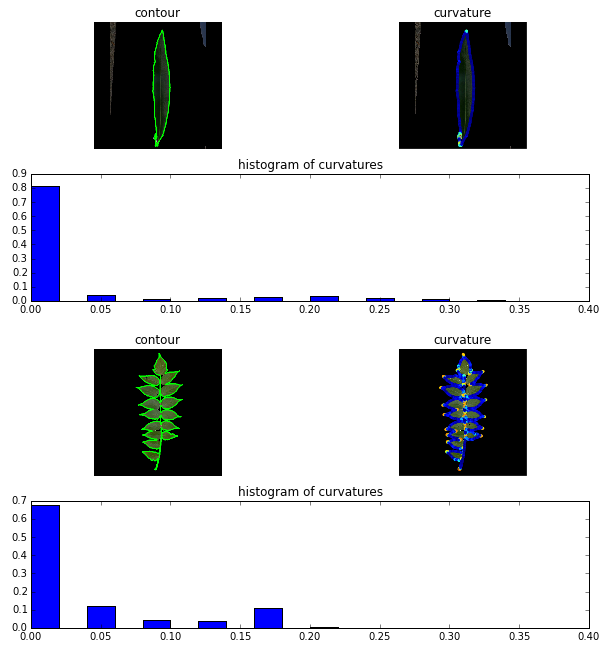
\includegraphics[width=0.6\linewidth]{img/curvatureHist.png}
  \caption{Histogrammes des courbures des images des feuilles 1 et 13}
  \label{curvaturehist}
\end{figure}


\section{Nouvelle caractéristique}

Dans l'exercice suivant, il est question d'extraire une nouvelle caractéristique pour l'ajouter au tableau de l'histogramme créé précédemment. Pour cela nous avons choisi d'extraire l'enveloppe convexe de la feuille et de la comparer avec le contour. La caractéristique est le coutour divisé par l'enveloppe convexe. Cette caractéristique est intéressante car plus la feuille est lisse et convexe, plus la caractéristique sera proche de 1 et plus il y a de renflements, plus la valeur va diminuer. Voici le code de la fonction qui va extraire cette caractéristique : 

\lstinputlisting{code/hull_ratio.py}


\section{KNN}

Il faut à présent utiliser les caractéristiques pour entraîner et évaluer un classificateur KNN. Pour ce faire, nous devons d'abord charger toutes les images et leur extraire les caractéristiques qu'on met dans un tableau. Il faut également créer un vecteur qui contient les classes de chaque image pour pouvoir entraîner notre classificateur. Ensuite nous séparons nos données en données d'entraînement et de test. A la fin, nous entraînons le classificateur. Voici le code qui permet toutes ces étapes : 

\lstinputlisting{code/knn.py}

Dans ce code, nous avons défini que 40\% des données allaient servir de données de test. Et nous avons instancié le classificateur KNN à K = 3. Nous pouvons changer la valeur de K pour voir si nous obtenons de meilleurs résultats. Nous avons testé avec les 1, 2, 3, 5 et 10 plus proches voisins et avons trouvé les valeurs qui se trouvent dans la table \ref{valuestabforKNN}.

\begin{table}[h]
  \centering
  \footnotesize
  \begin{tabular}{|c|c|c|c|}  
    \hline
    K & precision & recall & f1-score \\
    \hline
    1 & 0.86 & 0.86 & 0.86 \\
    2 & 0.84 & 0.84 & 0.83 \\
    3 & 0.87 & 0.87 & 0.86 \\
    \rowcolor{very-light-gray}
    5 & 0.88 & 0.87 & 0.86 \\
    10 & 0.82 & 0.86 & 0.84 \\
    \hline
  \end{tabular}
  \label{valuestabforKNN}
  \caption{Résultats pour différentes valeurs de K}
\end{table}

La ligne grise montre que la version 5NN est la meilleure dans les trois catégories \texttt{precision}, \texttt{recall (sensibility)} et \texttt{f1-score}. Voici donc les résultats complets que l'on a trouvé avec 5NN. La figure \ref{5nnconfusionmatrix} montre la matrice de confusion et la table \ref{5nnclassificationreport} montre le rapport de classification complet.

\begin{figure}[h]
  \centering
    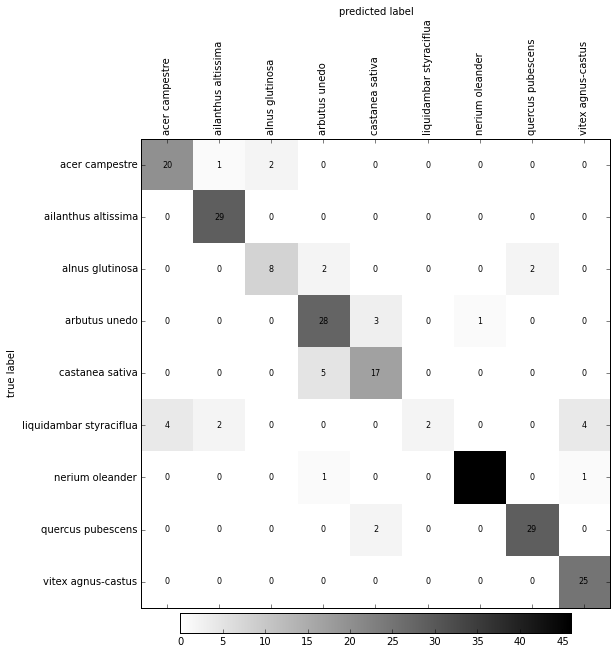
\includegraphics[width=0.6\linewidth]{img/5NN.png}
  \caption{Matrice de confusion pour 5NN}
  \label{5nnconfusionmatrix}
\end{figure}

\begin{table}[h]
  \centering
  \footnotesize
  \begin{tabular}{|r|r|r|r|r|}  
    \hline
    type & precision & recall & f1-score & support\\
    \hline
    acer campestre & 0.83 & 0.87 & 0.85 & 23\\
    ailanthus altissima & 0.91 & 1.00 & 0.95 & 29\\
    alnus glutinosa & 0.80 & 0.67 & 0.73 & 12\\
    arbutus unedo & 0.78 & 0.88 & 0.82 & 32\\
    castanea sativa & 0.77 & 0.77 & 0.77 & 22\\
    liquidambar styraciflua & 1.00 & 0.17 & 0.29 & 12\\
    nerium oleander & 0.98 & 0.96 & 0.97 & 48\\
    quercus pubescens & 0.94 & 0.94 & 0.94 & 31\\
    vitex agnus-castus & 0.83 & 1.00 & 0.91 & 25\\
    \hline
    avg / total & 0.88 & 0.87 & 0.86 & 234\\
    \hline
  \end{tabular}
  \label{5nnclassificationreport}
  \caption{Rapport de classification pour 5NN}
\end{table}

Pour information, voici les formules permettant de trouver les trois valeurs \texttt{precision}, \texttt{recall} et \texttt{f1-score} :

\[ precision = \frac{\sum TruePositive}{\sum TestOutcomePositive} \]

\[ recall = sensitivity = \frac{\sum TruePositive}{\sum ConditionPositive} \]

\[ f1-score = 2 \cdot \frac{precision \cdot recall}{precision + recall} \]

\newpage 

Nous essayons ensuite de ne pas tenir compte de la caractéristique \texttt{hull\_ratio} pour voir la différence dans les résultats. Nous relançons donc la simulation toujours en considérant les 5 plus proches voisins. La figure \ref{5nnwithouthull} montre la matrice de confusion résultante. Et la table \ref{5nncrwithouthull} montre les valeurs du rapport de classification.

\begin{figure}[h]
  \centering
    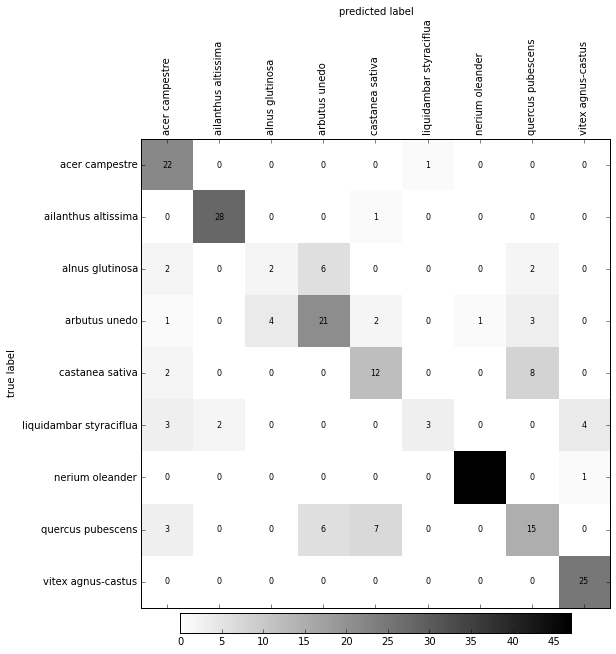
\includegraphics[width=0.6\linewidth]{img/5NNwithoutHull.png}
  \caption{Matrice de confusion pour 5NN sans la caractéristique \texttt{hull\_ratio}}
  \label{5nnwithouthull}
\end{figure}

\begin{table}[h]
  \centering
  \footnotesize
  \begin{tabular}{|c|c|c|}  
    \hline
    precision & recall & f1-score \\
    \hline
    0.74 & 0.75 &0.73 \\
    \hline
  \end{tabular}
  \label{5nncrwithouthull}
  \caption{Rapport de classification pour 5NN sans la caractéristique \texttt{hull\_ratio}}
\end{table}

Nous passons d'un t1-score de 86\% à 73\%. Nous pouvons donc affirmer que le choix de la caractéristique \texttt{ratio\_hull} était très bon et permet d'augmenter significativement la précision du classificateur.



% Code integration example
%\begin{lstlisting}[language=bash]
%  sudo apt-get update
%  sudo apt-get install drupal7
%\end{lstlisting}

% Image integration example
%\begin{figure}[h]
%  \centering
%    \includegraphics[width=1\linewidth]{img/drupalFirstPage.png}
%  \caption{Page d'accueil du site créé avec Drupal sur une instance EC2}
%  \label{drupalfirstpage}
%\end{figure}

% Image side-by-side
%\begin{figure}[h!]
%    \centering
%    \begin{tabular}{cccc}
%      \includegraphics[width=.14\linewidth]{randomTree_n5.png} &
%      \includegraphics[width=.22\linewidth]{randomTree_n10.png} &
%      \includegraphics[width=.22\linewidth]{randomTree_n15.png} \\
%      (a) & (b) & (c)\\
%    \end{tabular}
%    \caption{Arbres aléatoires où (a) n=5 (b) n=10 (c) n=15
%    \label{randomTrees}}
%\end{figure}
